\chapter{Materials and Methods} % Main chapter title

\section{Materials} 
\subsection{Yeast strains}
\begin{table}[H]
	\vspace*{-2.5cm}
	\hspace*{-1cm}%
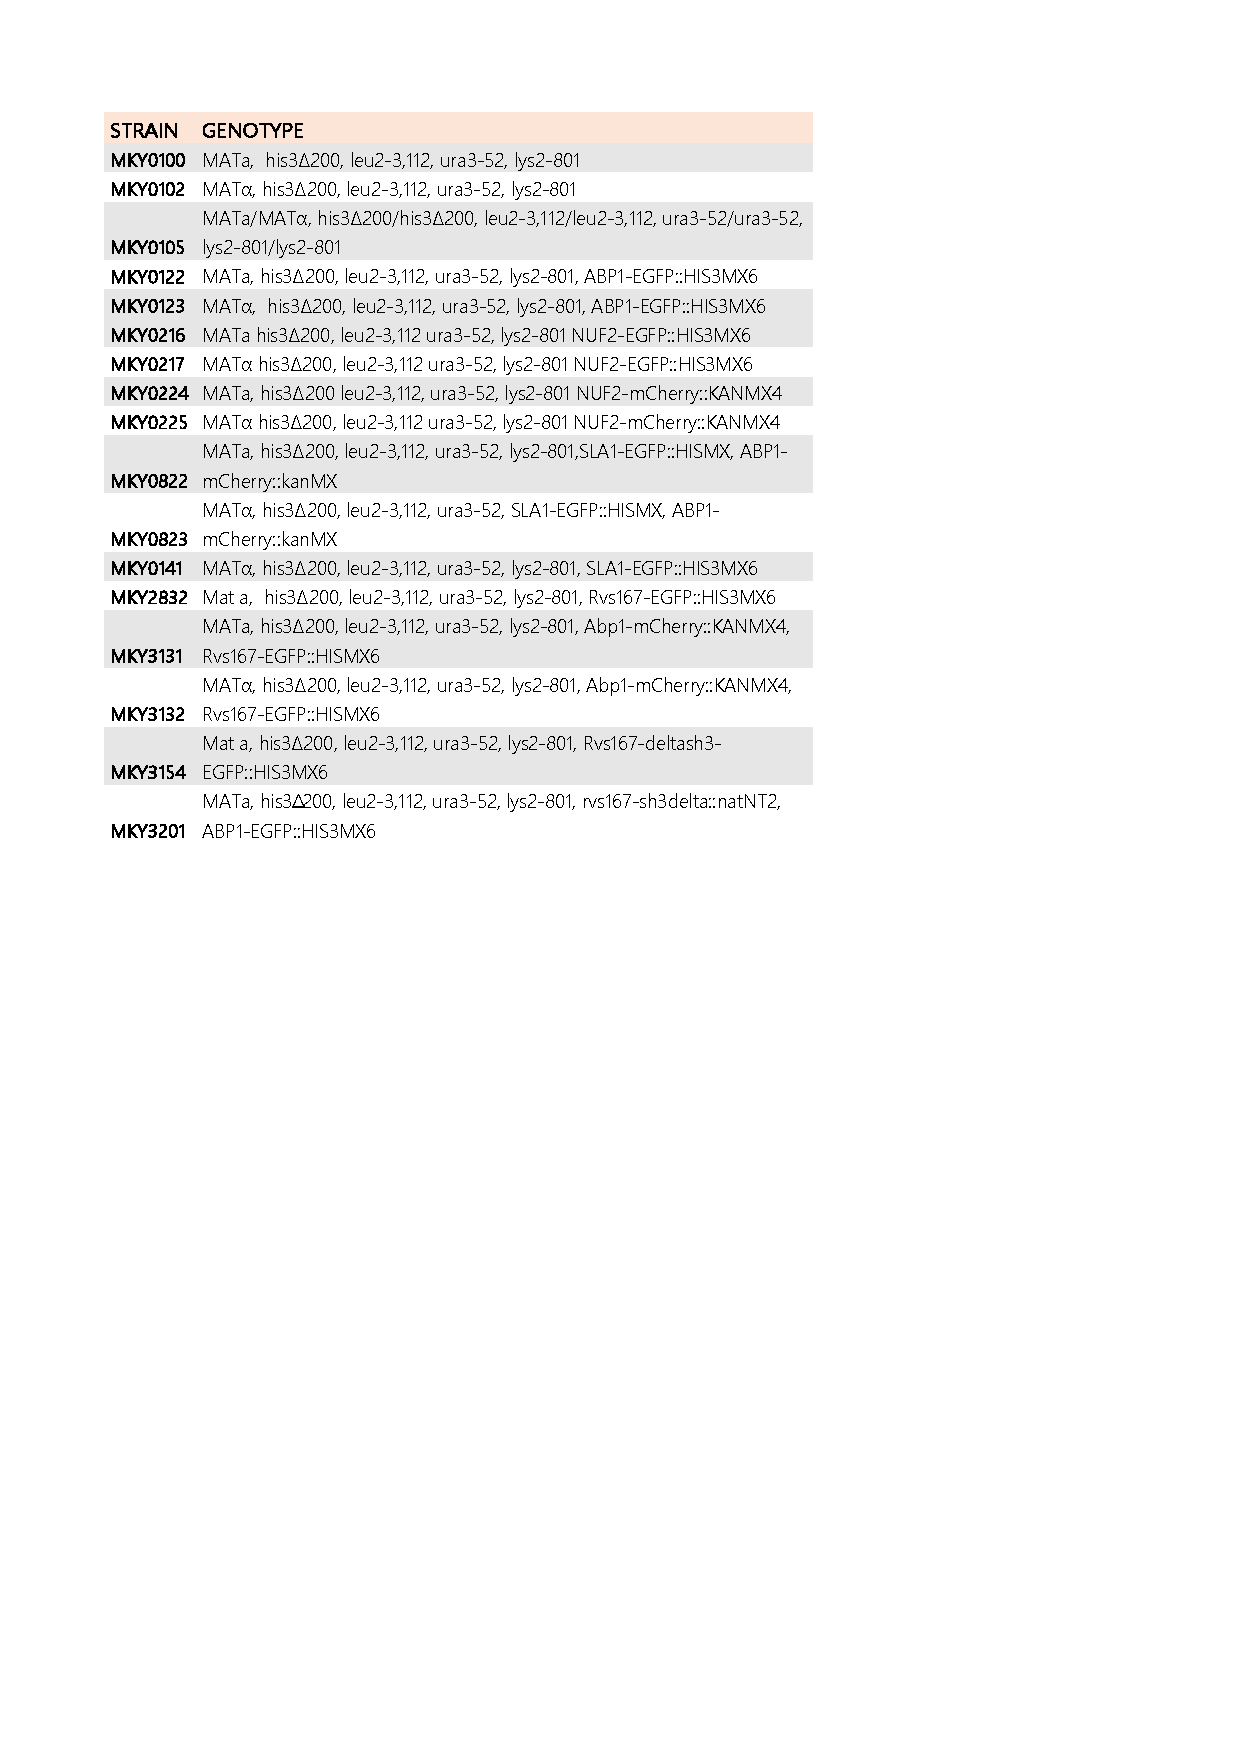
\includegraphics[width=35cm,height=35cm,keepaspectratio, valign=t]{figures/methods/strains_@1}
\caption[Yeast strains]

\end{table}


\begin{table}[H]
	\vspace*{-2.5cm}
	\hspace*{-2cm}%
	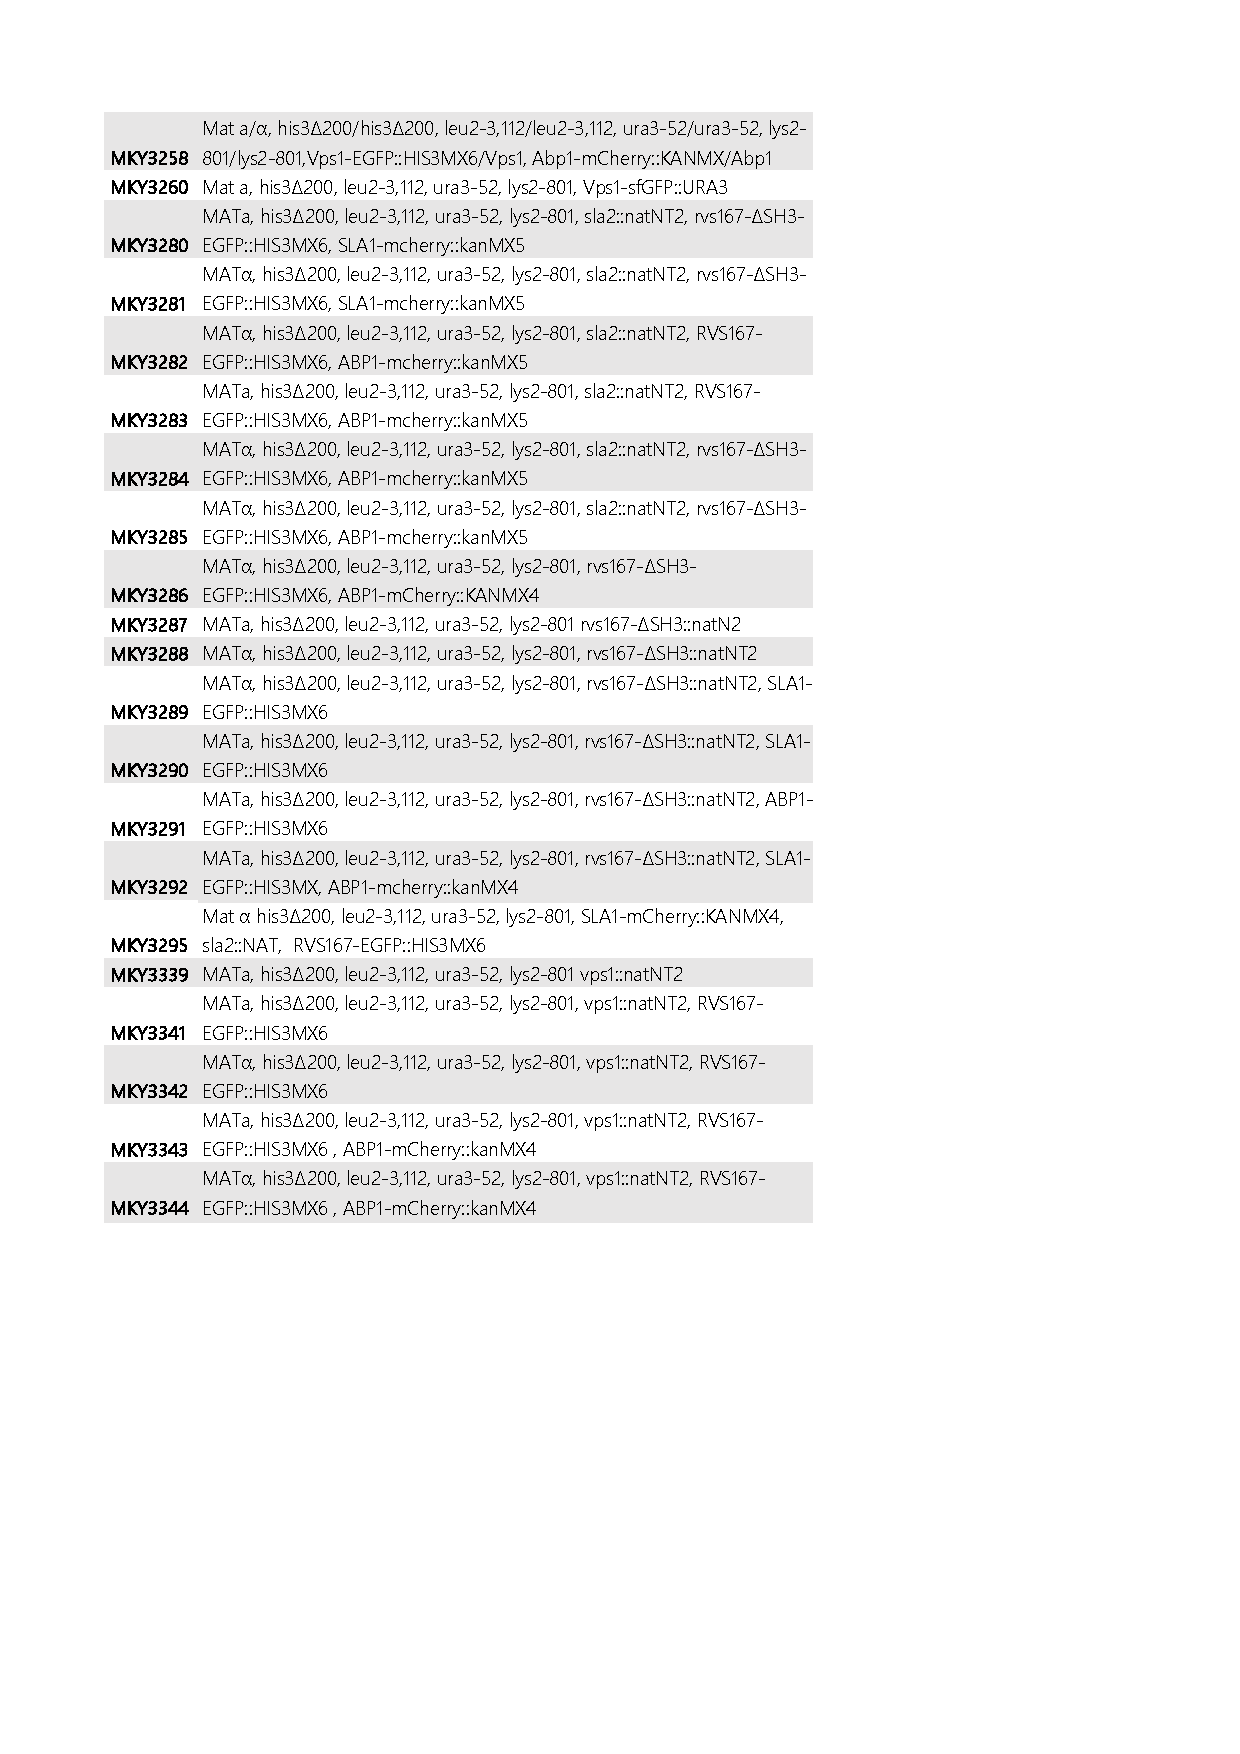
\includegraphics[width=35cm,height=35cm,keepaspectratio, valign=t]{figures/methods/strains_@2}
\end{table}

\begin{figure}[H]
	\vspace*{-2.5cm}
	\hspace*{-1cm}%
	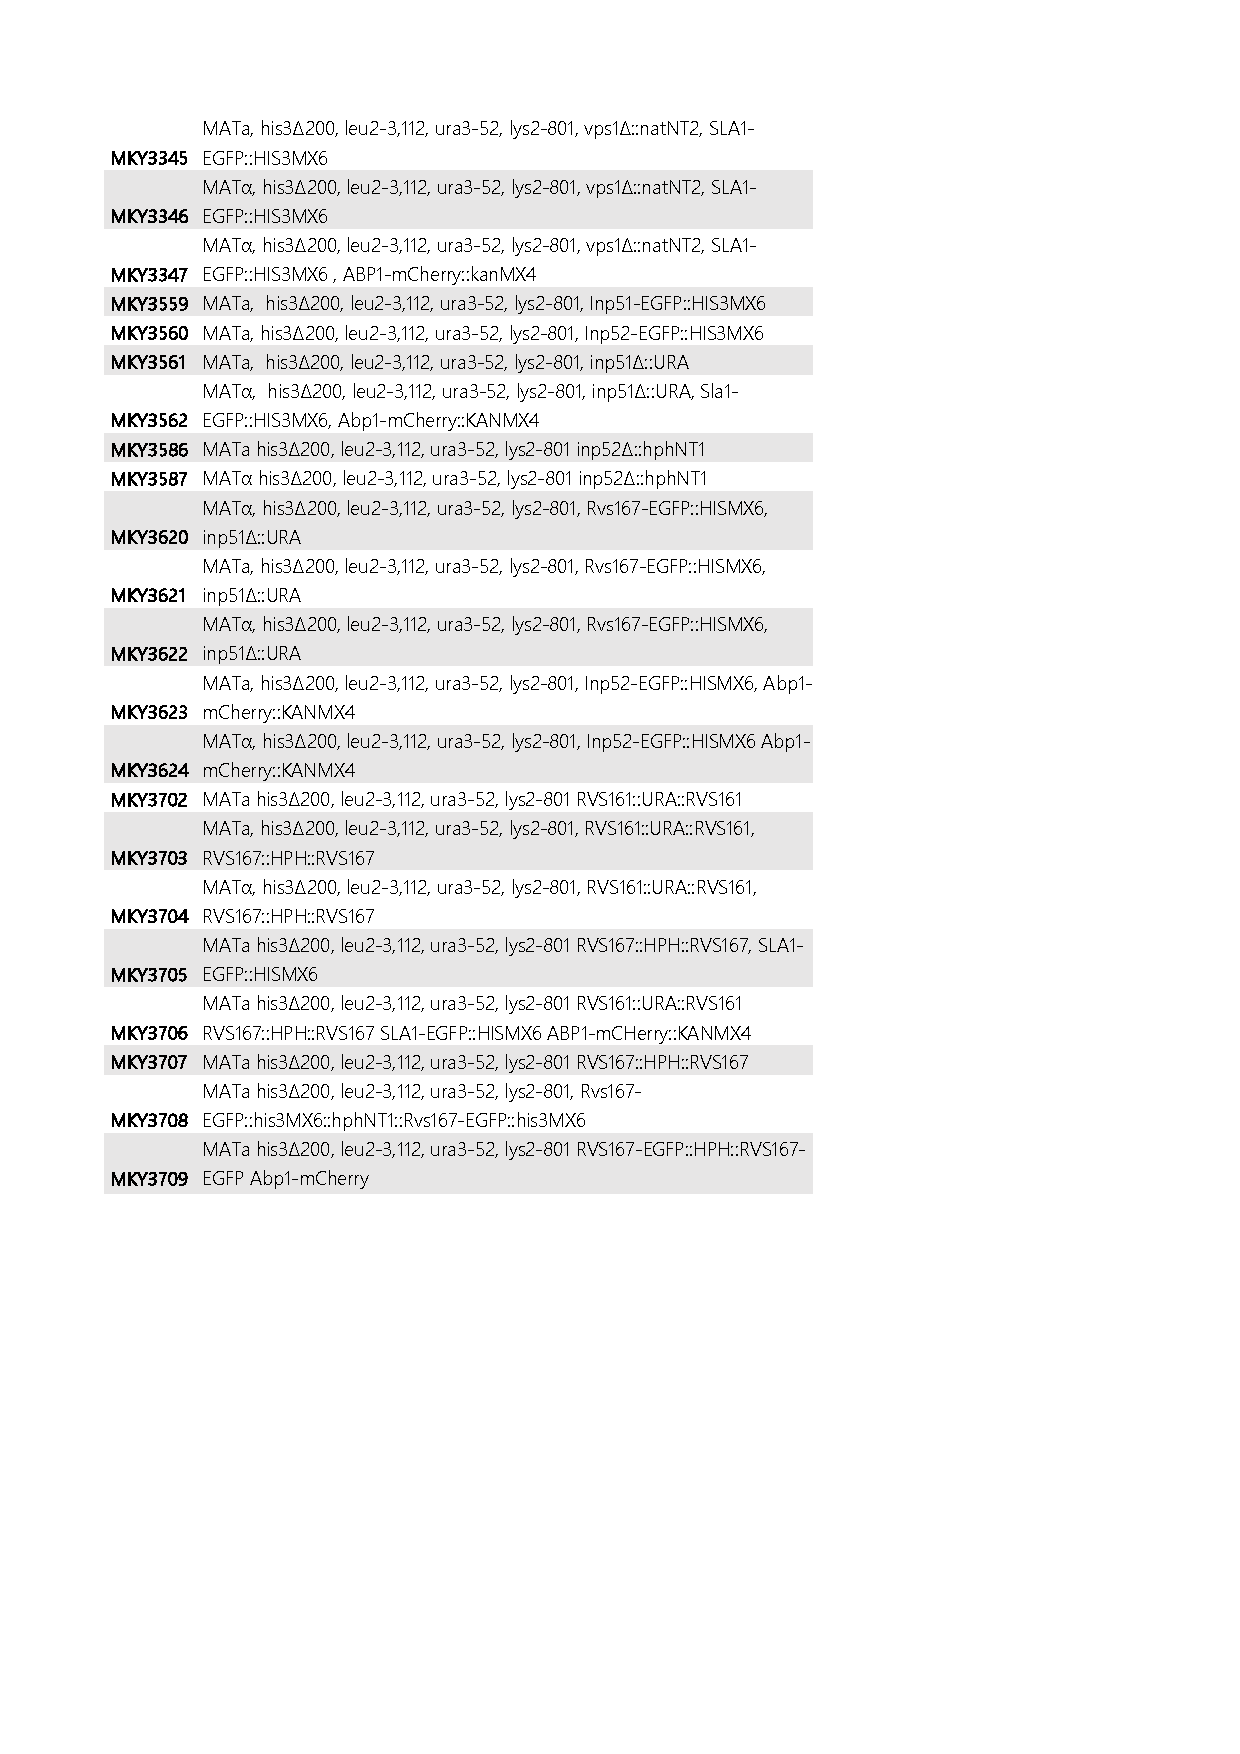
\includegraphics[width=35cm,height=35cm,keepaspectratio, valign=t]{figures/methods/strains_@3}
\end{figure}

\begin{figure}[H]
	\vspace*{-1.5cm}
	\hspace*{-2cm}%
	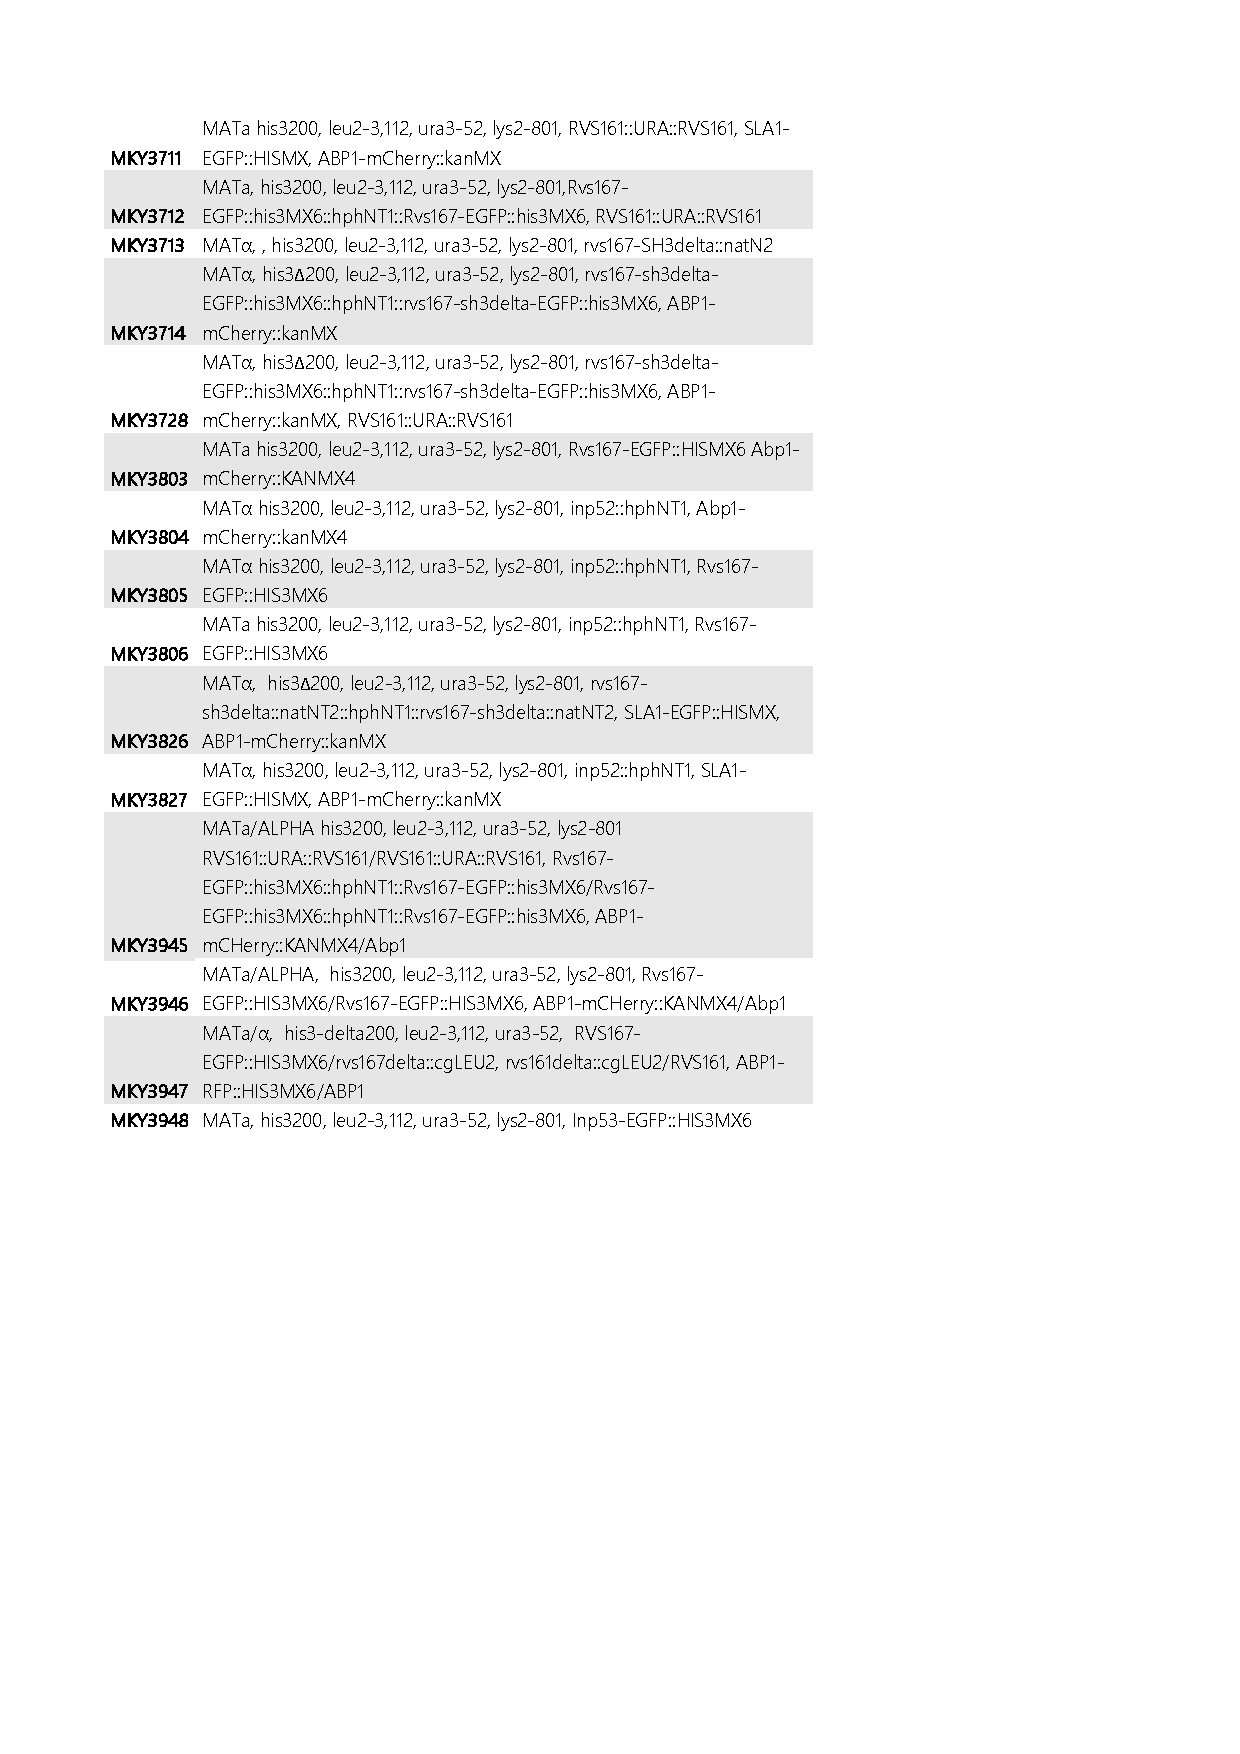
\includegraphics[width=35cm,height=35cm,keepaspectratio, valign=t]{figures/methods/strains_@4}
\end{figure}

\subsection{Media}
\begin{table}[H]
	\centering
	\vspace*{-1.5cm}
	\hspace*{-1.5cm}%
	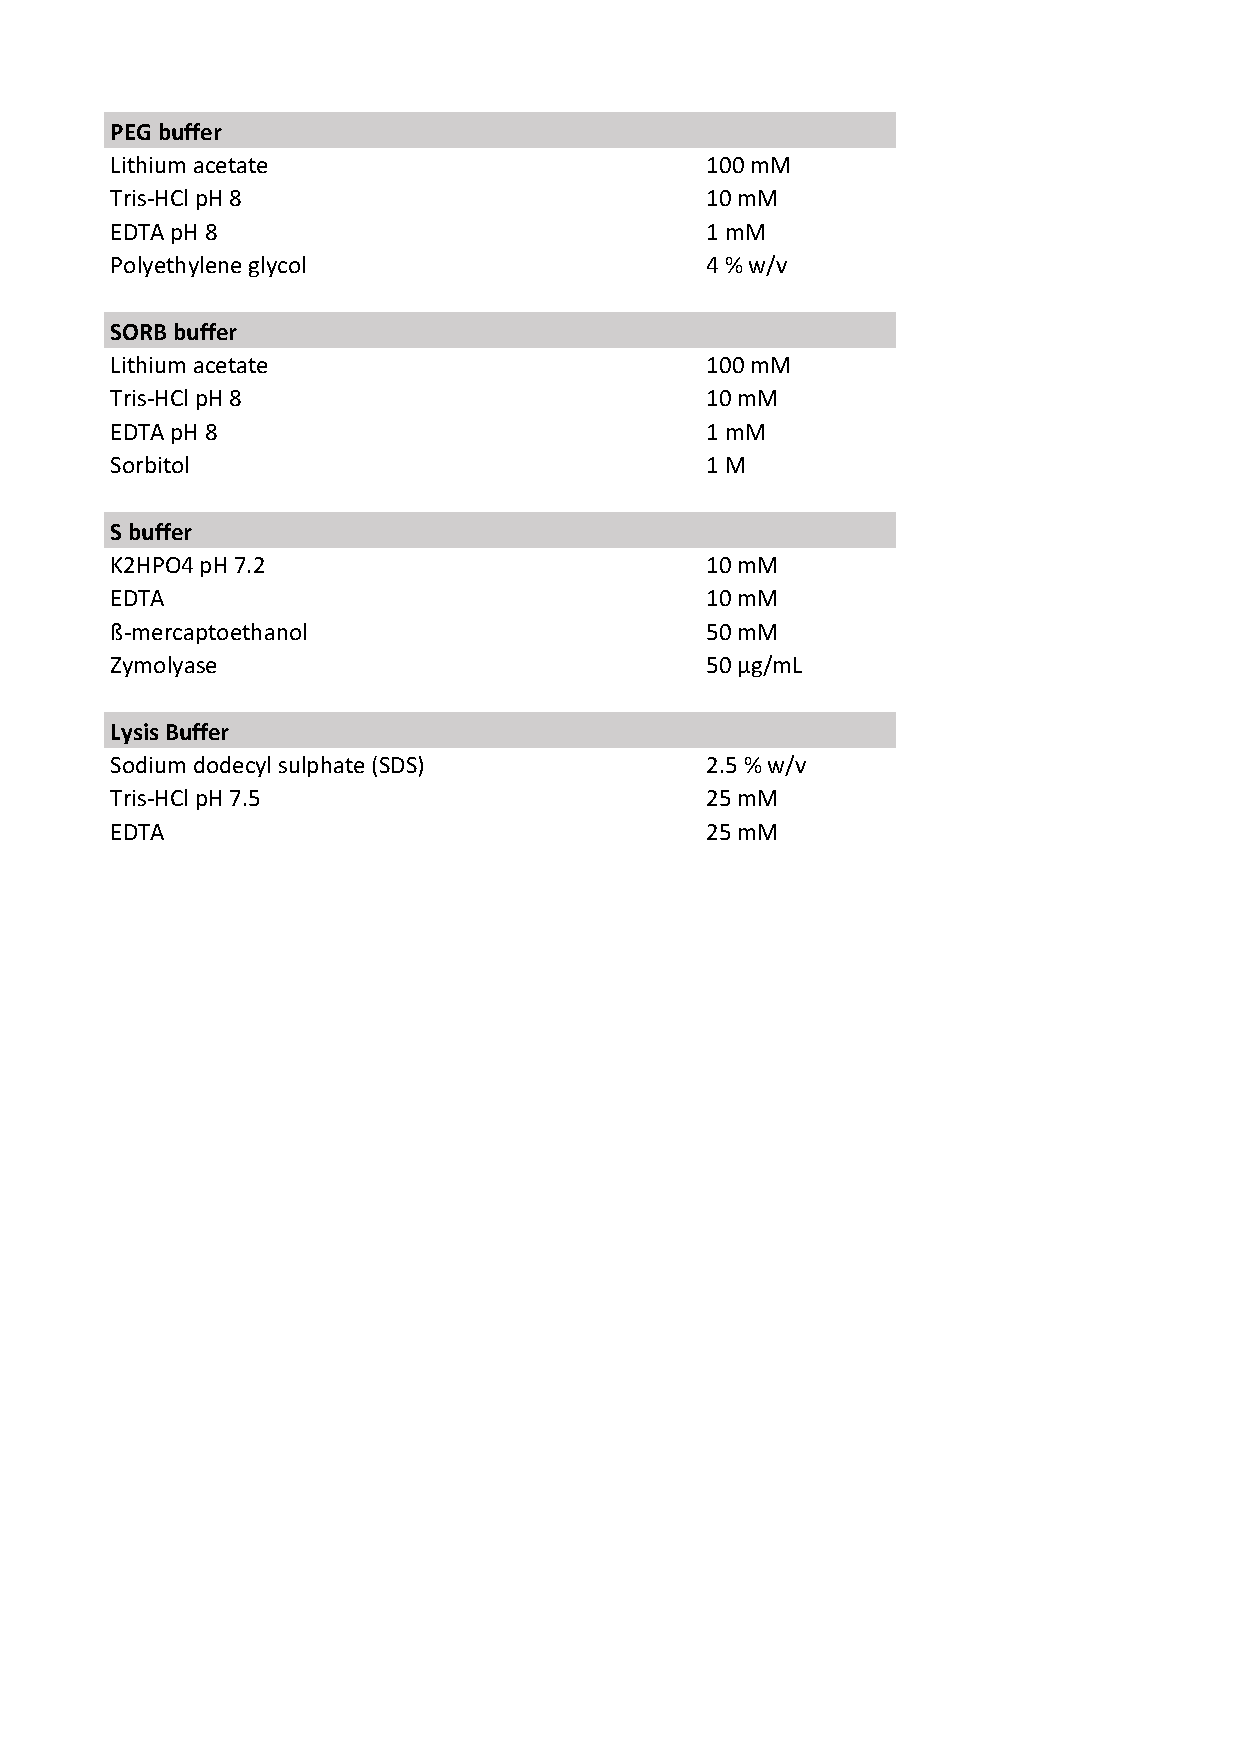
\includegraphics[width=24cm,height=24cm, keepaspectratio, valign=t]{figures/methods/Buffers}
\end{table}
other stuff happens

\section{Methods}
\subsection{Fluorescent tagging yeast with PCR casette insertion}
Tagging or deletion of endogenous genes was done by homologous integration of the product of a Polymerase Chain Reaction using appropriate primers and a plasmid containing a selection cassette and fluorescent tag, or only selection cassette for gene deletions. Primers were designed according to Janke et al, 2004. PCRs used the Velocity Polymerase for fluorescent tagging, and Q5 for gene deletions using the NAT casette. 
All fluorescently tagged genes have a C-terminus tag and are expressed endogenously.
Gene deletions and fluorescent tags are checked by PCR. Vps1del and gene duplications were confirmed by sequencing. 

\subsection{Live-cell imaging}
\subparagraph{Sample preparation for live imaging}
			\mbox{}\\
40 μL Concavalin A (ConA) was incubated on a coverslip for 10 minutes. 40 μL Yeast cells incubated overnight at 25C in imaging medium SC-TRP was added to the coverslip after removing the ConA, and incubated for another 10 minutes. Cells were then removed, adhered cells were washed 3x in SC-TRP, and 40 μL SC-TRP was finally added to the coverslip to prevent cells from drying. 

\subparagraph{Sample preparation for live imaging in LatA and Sorbitol treated cells}
\mbox{}\\
Cells went through the same procedure as above till the last washing step. Instead of SC-TRP, 100x diluted LatA, or Sorbitol at a final concentration of 0.2M in SC-TRP was added to the adhered cells. For LatA experiments, cells were incubated in LatA for 10 minutes before imaging. For sorbitol treatments, cells were imaged within 5 minutes of adding sorbitol.

\subparagraph{Epifluorescent imaging for centroid tracking}
			\mbox{}\\
Live-cell imaging was performed as in Picco et al. All images were obtained at room temperature using an Olympus IX81 microscope equipped with a 100×/NA 1.45 PlanApo objective , with an additional 1.6x magnification lens and an EMCCD camera. The GFP channel was imaged using a 470/22 nm band-pass excitation filter and a 520/35 nm band-pass emission filter. mCherry epifluorescence imaging was carried out using a 556/20 nm band-pass excitation filter and a 624/40 band-pass emission filter. GFP was excited using a 488 nm solid state laser and mCherry was excited using a 561 nm solid state laser. Hardware was controlled using Metamorph software. For single-channel images, 80-120ms was used as exposure time. All dual-channel images were acquired using 250ms exposure time. Simultaneous dual-color images were obtained using a dichroic mirror, with TetraSpeck beads used to correct for chromatic abberation.

\subparagraph{Epifluorescent imaging for molecule number quantification}
			\mbox{}\\
Images were acquired as in Picco et al. Z-stacks of cells containing the GFP-tagged protein of interest, incubated along with cells containing Nuf2-GFP, were acquired using 400ms exposure using a mercury vapour lamp, on a CCD camera. Z stacks were spaced at 200nm. 

\subparagraph{TIRF imaging}
			\mbox{}\\
TIRF microscopy was performed under similar conditions on an Olympus IX83 microscope. GFP was excited using a 488 nm solid state laser and mCherry was excited using a 561 nm solid state laser. Lasers, and shutters were controlled by Visitron Systems VS-Laser Control. VisiView software controlled the image acquisition and hardware-software feedback.
Images were processed using ImageJ, quantification was done on R.

\subsubsection{Live-cell Image analysis}
Images were processed for background noise using a rolling ball radius of 90 pixels. Particle detection, and tracking was performed for a particle size of 6 pixels, using scripts that combine background subtraction with Particle Tracker and Detector, that can be found on ImageJ (http://imagej.nih.gov). Further analysis for centroid averaging, alignments between dual-color images and single channel images, for alignment to the reference Abp1 were done using scripts written in Matlab (Mathworks) and R (www.r-project.org), written originally by Andrea Picco, and modified by me. Details of analysis can be found at Picco et al. All movement and intensity plots from centroid tracking show the average centroid with 95\% confidence interval. All molecule number quantifications report either the median or maximum number of molecules with standard error of mean. Maximum number is preferred over median in cases when the rate of change of fluorescent intensity of two populations being compared are not similar, and the lifetime of the protein populations being compared are not similar. The median in this case underreports the differences in protein accumulation. 


\subsubsection{CLEM}
Samples were prepared for CLEM as described in Wanda et al. Briefly, cells expressing Rvs167-GFP and Abp1-mCherry, and BAR-GFP and Abp1-mCherry cells were grown overnight in YPD, at 24C. They were then diluted to an OD600 of 0.2, and grown to OD600 between 0.8 and 1.2. These cells were then concentrated to a filter paper using a vacuum pump, and high-pressure frozen. Samples were freeze substituted in Lowycryl HM20 using the Kukulski freeze substitution protocol using an automated robot. 
\vspace{2mm}
Samples in resin were sliced to 300nm sections using a diamond knife, and loaded to carbon-coated copper grids. TetraSpec beads were incubated on the slices and these slices were imaged using epifluorescence microscopy in GFP and RFP channels for GFP and m-Cherry, and Cyan channel for separating the signal from the Tetraspec beads, that would later be used as fiducials to correlate these fluorescent images with electron tomograms. 
\vspace{2mm}
Gold fiducials were incubated on the grids, and lead citrate was added to stain the membrane. Low magnification tilts were acquired at 3 degree increments. High magnification tilts were perfomed at 1 degree increments from -60 to 60 degrees. Tomograms were reconstructed using IMOD. Invagination lengths were measured at the longest axis of the invagination, using IMOD.



